\documentclass{article}
\usepackage{header}

\title{\Huge{\textsc{heureka}}\\ \LARGE{02180 Introduction to Artificial Intelligence 2018}}
\author{Roar Nind Steffensen - s144107}
\date{May 2018}

\begin{document}

\maketitle

\tableofcontents

\vspace{2cm}

\section{Introduction}
In this \textsc{heureka} exercise I have designed, implemented and tested a heuristic search software system for route finding and resolution proving in the language \texttt{Java}.

Through this exercise I have become more acquainted with heuristic search algorithms, direct and computational logical deduction, as well as creating modular and reusable software designs.

The schemes used are guided by the text book \cite{ai_text_book} as well as the lectures. An framework is created with abstract classes with general notions of the graph search algorithm. These classes are extended to specify specific functionality for the task intended to be solved.

\pagebreak
\section{The Abstract Framework}
\subsection{Requirements}

Inspecting the \textsc{graph-search} algorithm specified in the book\cite{ai_text_book} section 3.3, we see that it requires the following elements:
\begin{itemize}
    \item \texttt{State}: Vertex in the graph / current system state
    \item \texttt{Action}: Edge in the graph / possible state transition
    \item \texttt{Result}: Return value
    \item \texttt{Problem}: What is intended to be solved
    \item \texttt{GraphSearch}: The search algorithm
\end{itemize}

Since the search algorithm described in the book is completely generic, and meant to be highly flexible, several design decisions has to be made in order to translate the elements into usable classes:

\texttt{State} is a data wrapper, meaning the only things we need from it is, access to the content, and a description as how to compare states, an addition to help create usable output the state also has a possible link to another state. 

\texttt{Action} is a relation between states. As we are working with graphs actions are binary (contains two states), and also contains a description as how to compare actions.

\texttt{Result} informs if the search was successful or a failure. As an addition the result value also contains the goal state. This makes it possible for the program to trail the found path using the links specified in the states.

\texttt{Problem} is perhaps the most abstract component from the \textsc{graph-search} algorithm specified in the book. What we need from this element, is the graph itself with states and actions, descriptions as how to navigate the graph, heuristics, the initial state and the goal state. 

\texttt{GraphSearch} contains the search algorithm specified in the book, extended to also be compatible with the A* algorithm, as described in exercises of week 6 of the course. What the element must contain to tailor the search algorithm to any graph search algorithm, is how to choose the next state from the frontiers, an evaluation function if the goal state is found, and a description of how two states are linked.


\subsection{Classes}

With the elements described in the previous section, we can create a complete abstract graph search framework to be used in a wide variety of scenarios. As the decisions and content has been largely outlined already, each of the elements are easily translated into classes. All classes will be abstract except the \texttt{Result} class. As this class will contain a \texttt{State} and a boolean expressing if the search was successful.\footnote{Technically the \texttt{Result} could deliver the same information with only the \texttt{State} stating if the search was successes based on a null-check on the state. A boolean is kept in this implementation however, as the user may utilize null states in their system.} 

Many of the descriptions mentioned in the requirements will be implemented as abstract methods, where the functionality and search specifics are specified by the extending class. Simple or optional methods such as getters/setters or the link/heuristic methods are not forced to be overwritten, as multiple scenarios don't need these to be tailored.

The resulting classes are seen in figure \ref{fig:framwork_classdiagram}.

\begin{figure}[H]
    \centering
    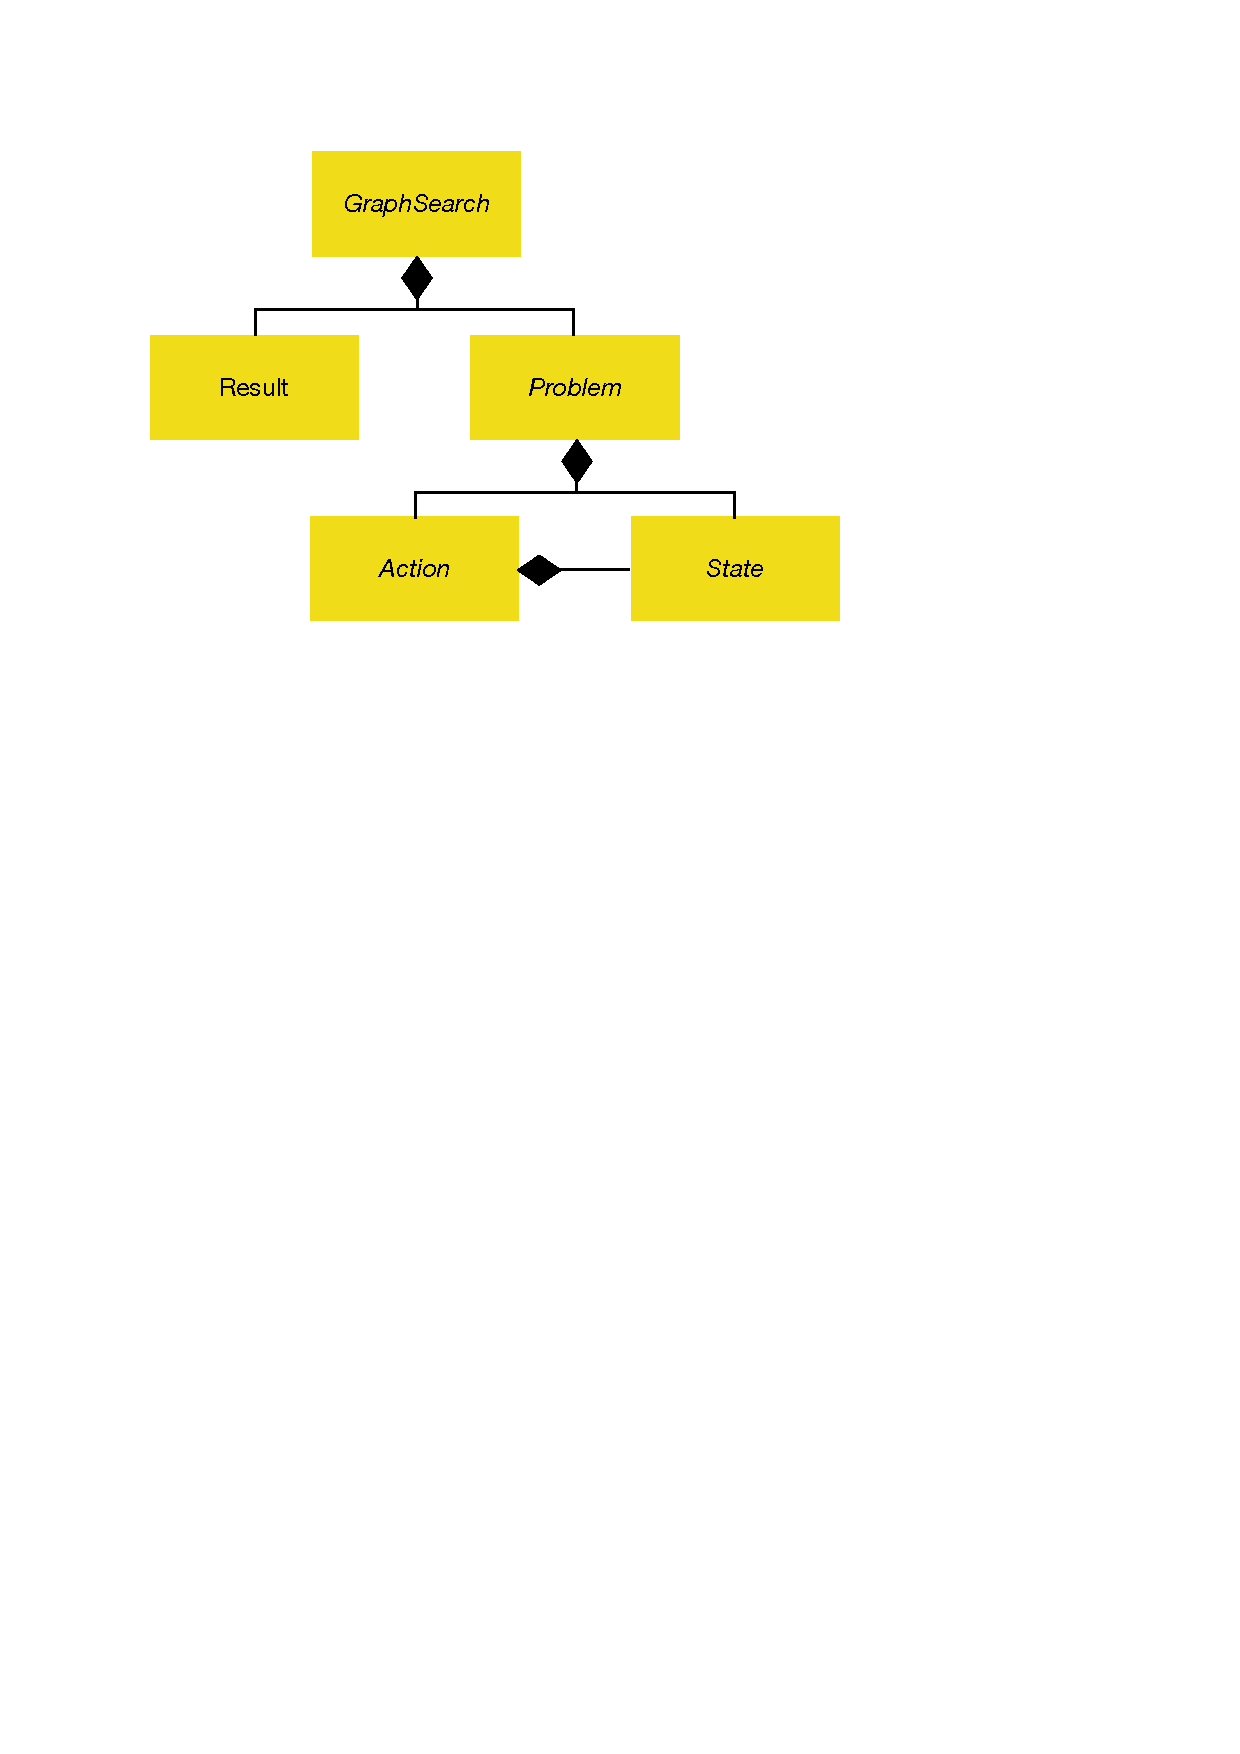
\includegraphics[width=0.6\linewidth]{FrameWork/AbstractFrameworkClassDiagram.pdf}
    \caption{Simple class diagram of the relationship between the framework classes.\protect\footnotemark}
    \label{fig:framwork_classdiagram}
\end{figure}

\footnotetext{Only the relations between the classes are shown in the class diagram to keep it clean, as the methods are described in the text above.}
\section{Route Finding}

For this part of the exercise we intend to implement a graph searching algorithm for route finding on a map. A series of data points are given for the exercise in form of a list of tuples, of size 3, with the needed map information. The tuples are in the form of:

\begin{equation} \label{eq:maptuple}
    (\text{start location} \star \text{road name} \star \text{end location})
\end{equation}
    
We see that the map is represented by a graph constructed by a series of edges. When constructing the graph, any uncharted location (start or end) constitutes a new vertex. As a map may contain one-way streets, the graph is not bidirectional, which is possible since the tuple information states the direction of the respective edges. A road which is not direction restricted will then be stated as two similar edges but with swapped start/end locations.

Initially the A* and the RBFS algorithms were implemented individually to solve the map search problem. But later only the A* was kept, as this is based on graph search, where RBFS is based on tree search. Since one of the main objectives with this exercise was to re-use modules, it seemed appropriate to go with A* graph search as the map was given as a graph. 


\subsection{Implementation}
To utilize the framework specified in the previous sections, we need to tailor the graph search to A*, by creating a class \texttt{AStar} extending \texttt{GraphSearch}. To create our data structures we also need to create the classes \texttt{Crossing}, \texttt{Street}, and \texttt{Map} extending \texttt{State}, \texttt{Action} and \texttt{Problem} respectively. Where the extended class contain the following augmentations:

\texttt{Crossing}: \\
As the parameters $f$, $g$, $h$ are needed for the A* algorithm, for each state, these are added, as well as the coordinates for the crossing. Comparisons between different crossings only evaluates coordinates. Methods called \texttt{getPath} and \texttt{backtrack} are added to calculate the found path using state links.

\texttt{Street}: \\
As the map is navigated using street names, a label is added to each street. Comparisons use start/end crossings as well as street name.

\texttt{Map}: \\
The map specifies how to navigate the graph by implementing the methods \texttt{expandState}, \texttt{heuristic}, and \texttt{initializeFrontier}. To expand the current state (crossing) all reachable crossings are found using the available directional streets. Since this is a map search, the heuristics in this case is naturally based on a euclidean distance function. In this scenario, the frontier is initialized by adding the initial state. Additional methods for creating the map, and retrieving map information are implemented, to ease usage.

\texttt{AStar}: \\
Since the class extends the \texttt{GraphSearch} class, the implementation is quite simple. Only three methods needs to be overwritten. To implement the A* algorithm, the next state chosen from the frontier, should be the state with the lowest $f$ value. The goal state/crossing evaluating uses the crossing comparison together with the specified goal state in the map. Here the link method is essential to finding the shortest path. The implementation links the new crossing the the previous, if it is a new crossing, or if it was previously evaluated with a longer path from the initial state.\footnote{This linkage is much similar to the proposed implementation from week 6 exercises with Thomas Bolander.}


\subsection{Testing}

\begin{multicols}{2}


With the proposed implementation of the framework, we get the following search results given the "city map data set" test data. Which can be seen on the right. 

As the map is to scale with the given locations, street names are quite small, but when viewed on a device, it should be possible to zoom in and view details if interested.

For testing, it will be interesting to see if directional uni-directional streets are respected, as well as if the map finds the shortest path if possible.

First, we can try to check if the algorithm can find the trivial path from a crossing to the same crossing. As an example, the initial and goal crossing is set to be the crossing between "Vestervoldgade" and "Vestergade". The expected output from here should be an empty list of street names, as no street is needed to be travelled to reach the destination. This matches the actual output, as seen in figure \ref{fig:test1}.

\begin{figure}[H]
    \centering
    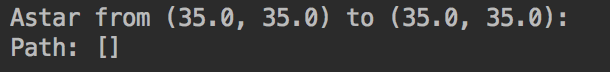
\includegraphics[width = 0.9\linewidth]{RouteFinding/RFtest1.png}
    \caption{Trivial route from crossing to same crossing result.}
    \label{fig:test1}
\end{figure}


\begin{figure}[H]
  \begin{center}
    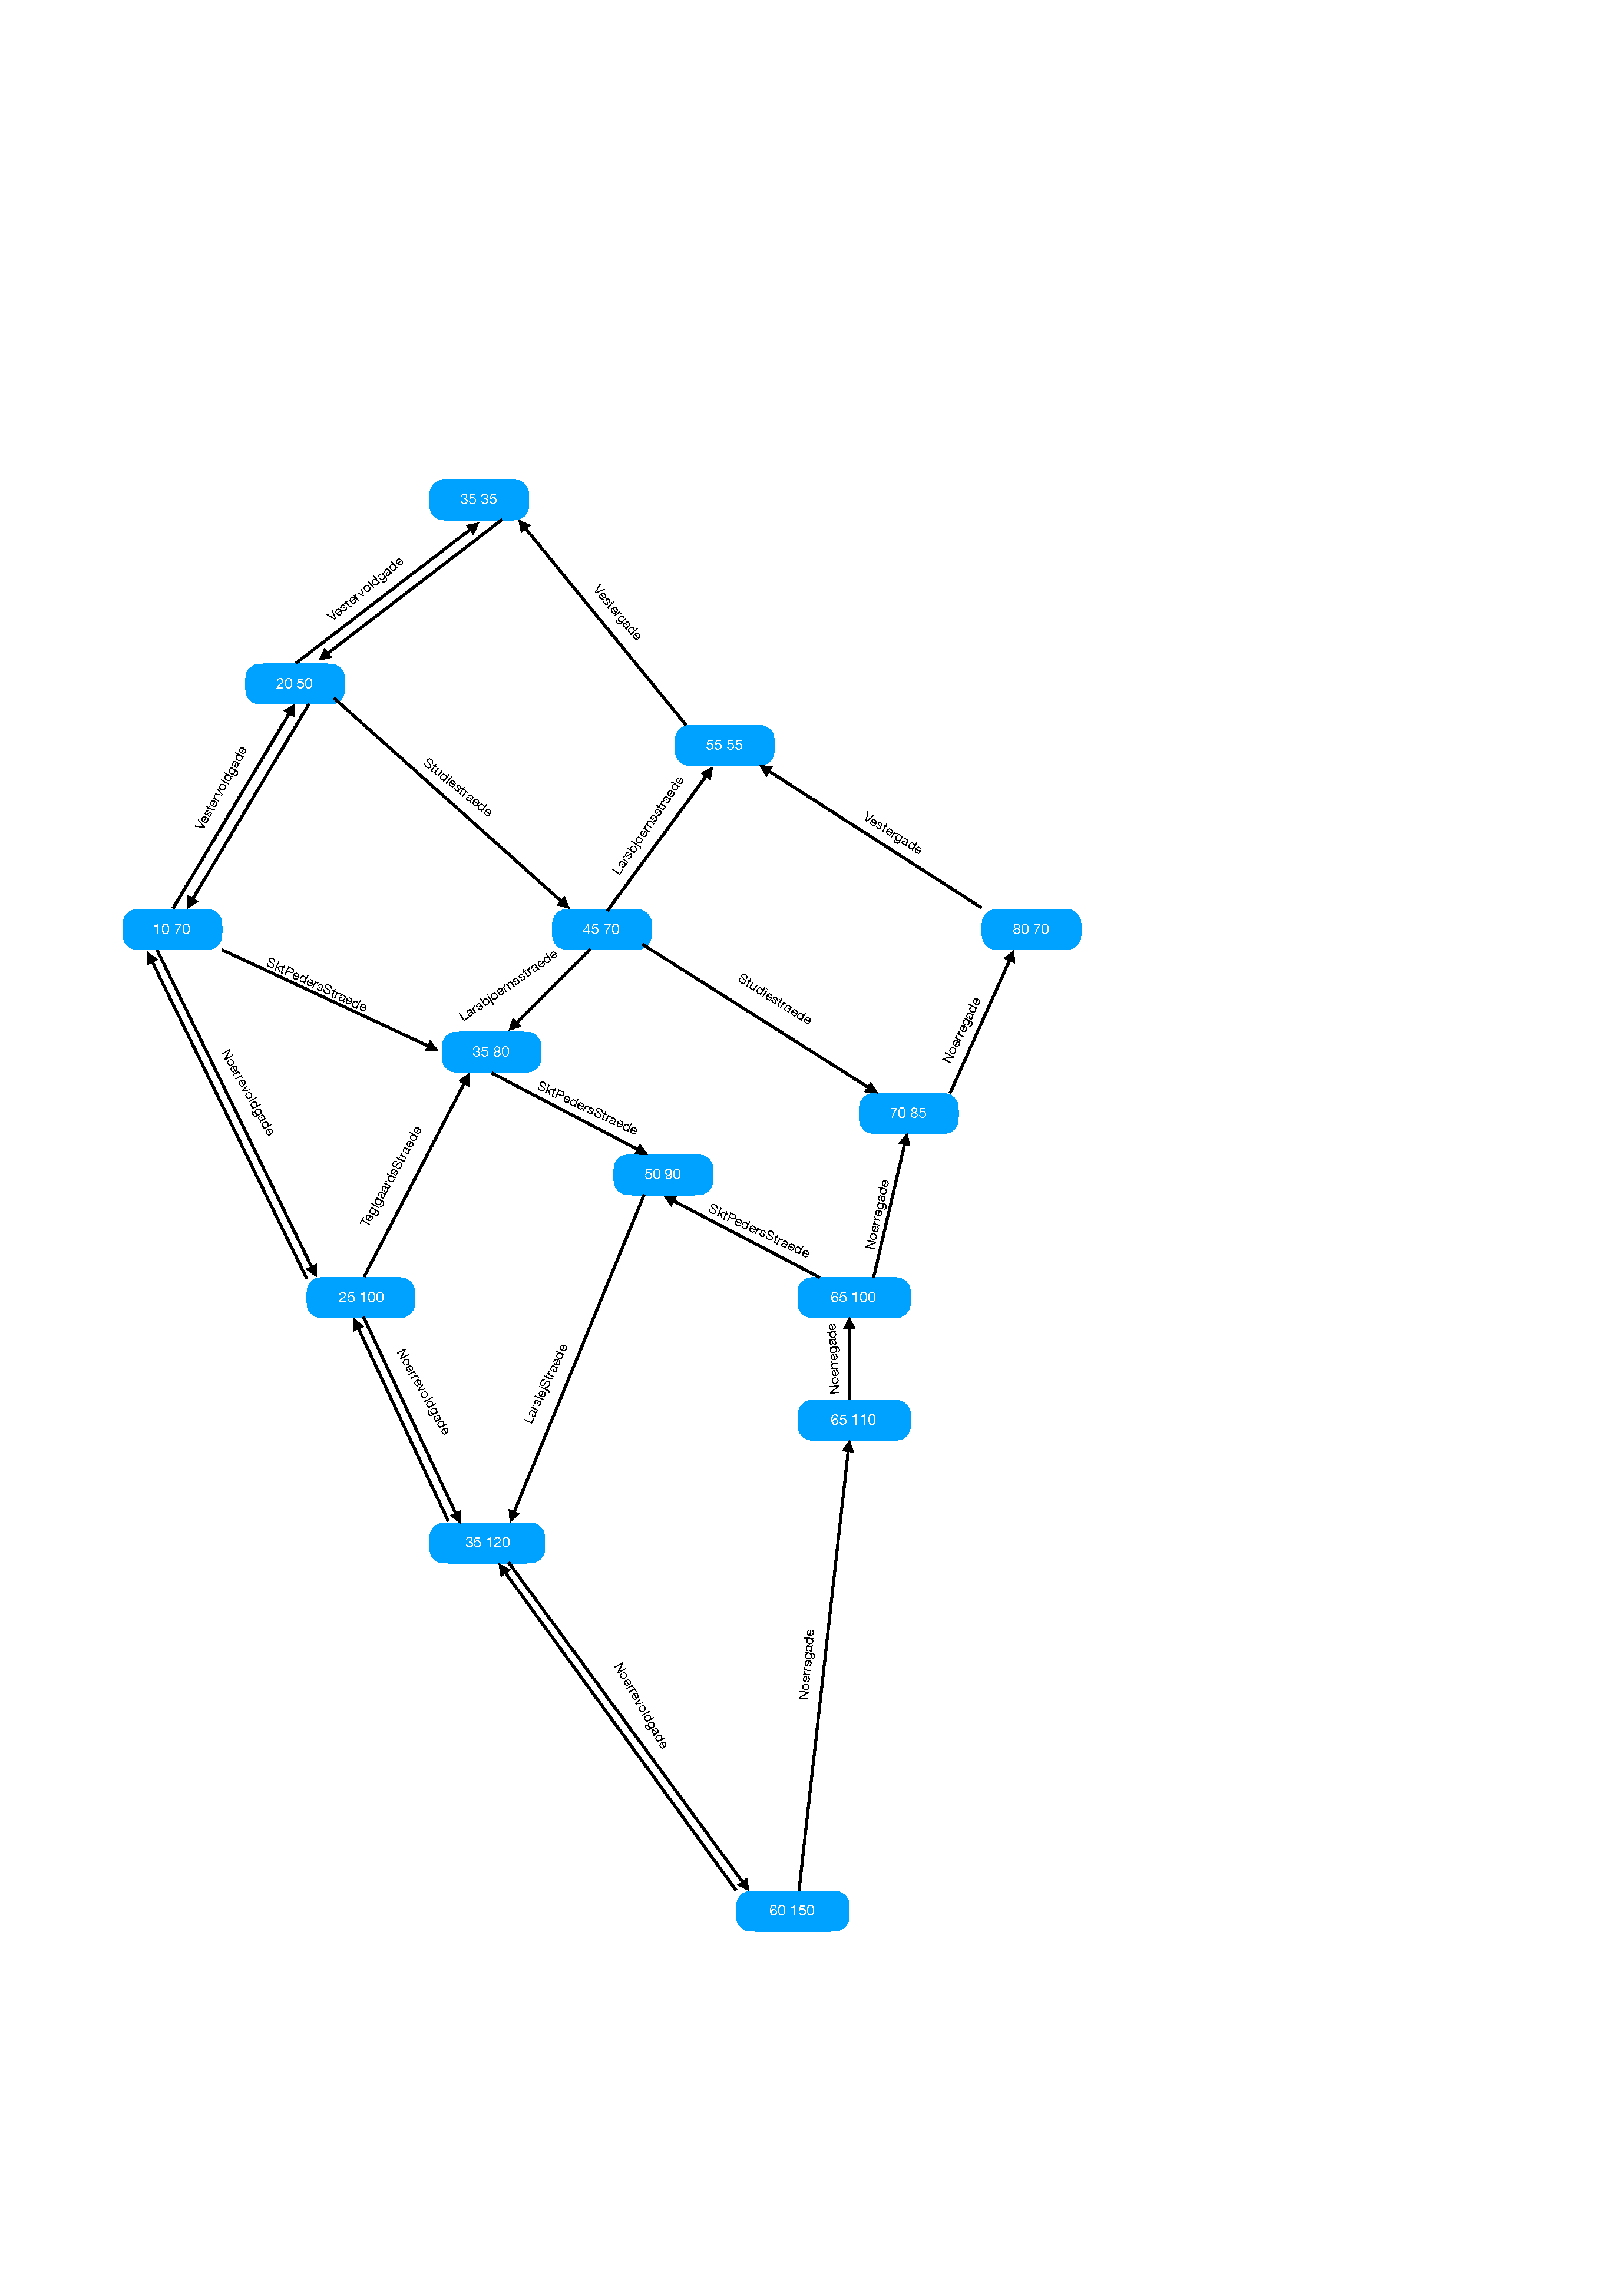
\includegraphics[width=0.9\linewidth]{RouteFinding/CityMap.pdf}
  \end{center}
  \caption{City Map}
\end{figure}

\end{multicols}

Next we test if the algorithm respects uni-directional streets. The example here is from the crossing between "Noerregade" and "Studiestraede", to the crossing between "Studiestraede" and "Larsbjoernsstraede". The expected output is, the path all the way around following the streets "Noerregade", "Vestergade", "Vestervoldgade" and "Studiestraede". This matches the actual output as seen in figure \ref{fig:test2}. Note that "Vestergade" is listed twice, as two travels along that street is performed.

\begin{figure}[H]
    \centering
    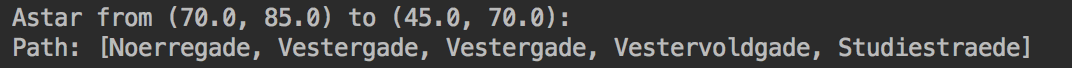
\includegraphics[width = 0.8\linewidth]{RouteFinding/RFtest2.png}
    \caption{Uni-directional street test result.}
    \label{fig:test2}
\end{figure}

Finally we want to test a route which has multiple possible paths, and verify that the output corresponds with the shortest possible path. The example here is from the crossing between "Vestervoldgade" and "Studiestraede", to the crossing between "SktPedersStraede" and "Noerregade".

Possible paths are and lengths are: \\
 $[$ "Vestervoldgade", "Noerrevoldgade", "Noerrevoldgade", "Noerrevoldgade", "Noerregade", "Noerregade" $]$
with a length of 157.62

$[$"Studiestraede", "Larsbjoernsstraede", "SktPedersStraede", "LarslejStraede", "Noerrevoldgade", "Noerregade", "Noerregade"$]$ 
with a length of 187.00

$[$"Vestervoldgade", "SktPedersStraede", "SktPedersStraede", "LarslejStraede", "Noerrevoldgade", "Noerregade", "Noerregade"$]$
with a length of 190.22

We expect to see the first path as output. This matches the actual output as seen in figure \ref{fig:test3}.

\begin{figure}[H]
    \centering
    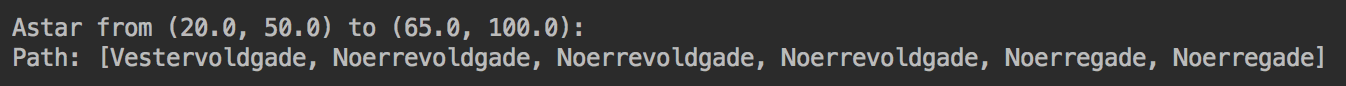
\includegraphics[width = 0.9\linewidth]{RouteFinding/RFtest3.png}
    \caption{Shortest path test result.}
    \label{fig:test3}
\end{figure}

Based on these tests, it is probable that the implementation of the A* algorithm is correct, as it has satisfied our behavioral expectations.
\section{Inference Engine for Propositional Logic}

Next we wish to use the graph search approach to proving a propositional logic formulated clause given a knowledge base. To conduct the proof, the search algorithm utilizes resolution inference rule to construct a refutation proof. The approach is much similar to a forward chaining algorithm, but creating the new statements through resolution inference based on the previous statements.\footnote{The word 'statement' is used here instead of clause as the forward chaining algorithm introduced in this cause was based on if-rules and not necessarily in clausal normal form (CNF).}

To construct the refutation proof, we negate the initial hypothesis (the hypothesis which we wish to proof is entailed by the knowledge base), and search for a contradiction between the negated hypothesis and the knowledge base.

When searching we know that we have met a contradiction when 
\subsection{Implementation}

Much like before, we need to extend the base classes from the framework. This time we create the classes \texttt{Clause}, \texttt{KnowledgeBase} and \texttt{RefutationProver}, extending the classes \texttt{State}, \texttt{Problem} and \texttt{GraphSearch}. A second data class \texttt{Literal} is also created, to break up clauses easier. Here the classes contain the following specifications:

\texttt{Literal}: \\
The literal is the most atomic data type in the data structure. It is composed of an atomic unit and a boolean expressing if it is negated or not. Other methods are \texttt{equals} and \texttt{toString} used for comparisons and overview respectively.

\texttt{Clause}: \\
The clause is a conjunction of disjunctions of literals. Here the knowledge base is a conjunction of clauses, meaning also a conjunction of disjunctions. To simplify things, we keep the clause as a list of literals, which are interpreted as disjunctions. This way the clause and literal accessibility is straight forward. The only limitation is, that the input to the program is constrained to a list of disjunctions. Based on the 'Clauses' section of the exercise description, and the statement "any clause $L_1$ v $L_2$ v ... v $L_{l+k}$", the clauses consist of a sequence of literals, which here are depicted as disjunctions. 

The \texttt{Clause} class has methods mainly for comparison (independent of literal sorting) and removing duplicate literals.

\texttt{KnowledgeBase}: \\
Since we don't specify relations between clauses, the \texttt{Action} class is not extended. This means that more work is done during the \texttt{expandState} method. Here the first clause from the list is chosen and combines with each of the other clauses testing for resolution, creating a list of new clauses. The initialization of the frontiers for the \textsc{graph-search} is also quite different, since it is initialized by adding all known clauses (included the negated hypothesis) to the list. The negation of the hypothesis is done by using De Morgan's law for negation of disjunctions, creating a conjunctions of negations, each added to the set of clauses in the knowledge base.

\texttt{ResolutionProver}: \\
Again, using the framework, the actual algorithm has only small adaptations to make the search algorithm function. No heuristics are used in this example, and the next state is simple the first from the list, similar to the forward chaining algorithm. Testing for goal state is simply by testing that the clause is empty, since this is what constitutes the contradiction.
\subsection{Testing}

This time, we have to build up a knowledge base, and check the the proposed hypothesis is entailed from the knowledge base. Like before, we will start by a trivial test, checking if the proposition 'a' is entailed by a knowledge base consisting of the clause 'a'. We expect the proof to be successful. This matches the actual output, as seen in figure \ref{fig:RPtest1}.

\begin{figure}[H]
    \centering
    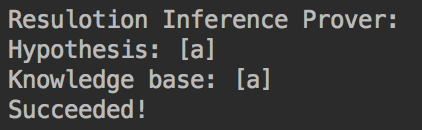
\includegraphics[width=0.3\linewidth]{ResolutionProver/RPtest1.png}
    \caption{Trivial refutation proof test result.}
    \label{fig:RPtest1}
\end{figure}

Next we test an implication in CNF. The example here contains 'not a or b' in the knowledge base, and 'a' as the hypothesis, and we wish to see if it entails 'b'. This matches the actual output, as seen in figure \ref{fig:RPtest2}.

\begin{figure}[H]
    \centering
    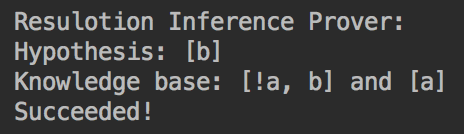
\includegraphics[width=0.3\linewidth]{ResolutionProver/RPtest2.png}
    \caption{Refutation proof for implication test result.}
    \label{fig:RPtest2}
\end{figure}

Finally we want to test if it correctly identifies when something is not entailed by the knowledge base. The example here contains 'a or b' in the knowledge base and 'a' as the hypothesis. We expect this to be 'not proven', as the knowledge base does not contain enough enough information to entail the hypothesis. This matches with the actual output, as seen in figure \ref{fig:RPtest3}.

\begin{figure}[H]
    \centering
    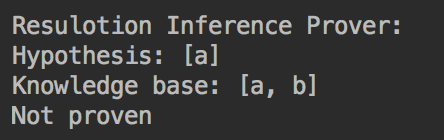
\includegraphics[width=0.3\linewidth]{ResolutionProver/RPtest3.png}
    \caption{Refutation proof where hypothesis does not entail from the knowledge base.}
    \label{fig:RPtest3}
\end{figure}

Based on these tests, it is probable that the implementation of the inference engine for propositional logic is correct,as it has satisfied our behavioral expectations.
\section{Summary and Conclusion}

Based on the A* implementation and the inference engine implementation of the abstract \texttt{graph-search} framework, the correctness and ease of use has been satisfying and interresting to work with. 

Both implementations worked successfully, and the framework is deemed flexible and highly re-usable, as minimal implementation was needed when extending the framework for specific purposes, even through the two use cases used in this exercise alone were quite different. A substantial part of the specific implementations were for usability when testing the search algorithms, meaning it does not take much to run the algorithm itself.

For future work, it would be interesting to create the corresponding abstract framework for tree search, and testing e.g. RBFS instead of A*.
\vfill
\printbibliography
\end{document}
